\section{Message broker}
\subsection{Descrizione generale}
Un \textit{message broker} è un software che permette di fare interagire varie applicazioni in
un contesto distribuito. Il suo compito principale è permettere a servizi eterogenei di comunicare con successo.
Viene solitamente utilizzato per la comunicazione fra microservizi in una architettura distribuita
e per operazioni che richiedono molto tempo in modo da ridurre il carico di lavoro sul web server.

Nel dettaglio un \textit{message broker} è un software che implementa il paradigma \textit{Message Oriented Middleware} (MOM) e offre servizi per distribuire i messaggi (routing e politiche di recapito).
Ciò significa che verrà usato come \textit{gateway} di livello applicativo in un sistema in cui le applicazioni comunicano utilizzando messaggi
che vengono inseriti in code e dove vengono utilizzati dei nodi di smistamento per distribuirli verso la destinazione.
Questa tipologia di sistemi è detta \textit{message-queuing system} \cite{MessageBroker-Book} in cui è garantita la persistenza
grazie all'utilizzo delle code e la possibilità di creare topologie punto-punto o punto-multipunto con in nodi di smistamento.
In particolare avremo che il \textit{message broker} riceve dei messaggi da applicazioni dette \textit{publishers} e li indirizzerà verso applicazioni dette \textit{consumers} che processeranno questi messaggi.

Nella piattaforma è stato deciso di utilizzare un broker RabbitMQ \cite{rabbitMQ} usando come protocollo di messaggistica l'\textit{Advanced message Queuing Protocol 0-9-1}(AMQP) \cite{amqp},
per permettere alla API d'interagire con il microservizio del Mailer.

\subsection{Protocollo di messaggistica}
L'AMQP 0-9-1 è un protocollo di livello applicativo che permette a delle applicazioni client d'interagire con i \textit{message broker}.
Per rendere completa questa interazione è necessario che fra le parti venga specificata la sintassi da usare e la semantica dei messaggi per i servizi offerti dal broker.
Il protocollo AMQP li definisce entrambi:
\begin{itemize}
    \itemsep0em
    \item \textit{Advanced Message Queuing protocol} (AMQP): è il protocollo che definisce la sintassi dei messaggi che permettono ai client d'interagire con il broker.
    \item \textit{Advanced Message Queuing model} (AMQ model): definisce un insieme di elementi e standard che devono essere implementati dal broker in modo tale da supportare le interazioni fra \textit{publishers} e \textit{consumers}.
\end{itemize}

Il protocollo AMQP è un protocollo di livello applicativo diviso in due layer:
\begin{itemize}
    \itemsep0em
    \item \textit{Functional Layer}: definisce i comandi che permettono alle applicazioni di svolgere operazioni sul broker
    \item \textit{Transport Layer}:  gestisce il multiplexing del canale, il framing, la codifica e il trasporto dei messaggi. Permette anche la gestione degli errori, la comunicazione asincrona e funzionalità di heartbeat.
\end{itemize}

Il modello AMQ definisce tre tipologie di componenti, che vengono poi connessi e processati dal broker per erogare i servizi richiesti.
Nel dettaglio:
\begin{itemize}
    \itemsep0em
    \item \textit{Exchange}: componente che indirizza i messaggi alle code
    \item \textit{Message queue} ("coda di messaggi"): una struttura dati che memorizza i messaggi
    \item \textit{Binding}: regola che definisce la relazione tra l'\textit{exchange} e la coda.
\end{itemize}

\begin{figure}[h]
    \centering
    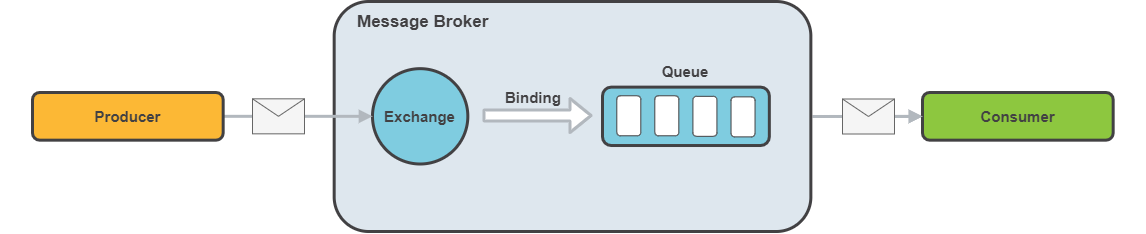
\includegraphics[scale=0.385]{amqModel.png}
    \caption{Modello AMQ}
    \label{fig:AmqModel}
\end{figure}


\subsection{Principi di design}
Nella piattaforma è stato utilizzato un broker RabbitMQ per supportare l'interazione tra API e Mailer e
disaccoppiare la fase di gestione della richiesta utente dalla fase di renderizzazione e invio email al destinatario.
Vista la possibilità di dover gestire numerose email contemporaneamente, è stato deciso di utilizzare il modello a \textit{consumers} concorrenti (\textit{Competing Consumers Pattern}) \cite{CompetingConsumers}.
Questo prevede la creazione di molteplici \textit{consumers} collegati a uno stesso canale in modo tale che questi possano processare più messaggi contemporaneamente.
Quando un messaggio arriva sul canale, uno qualsiasi dei \textit{consumers} potrebbe riceverlo e processarlo andando così a competere l'uno con l'altro.

\begin{figure}[h!]
    \centering
    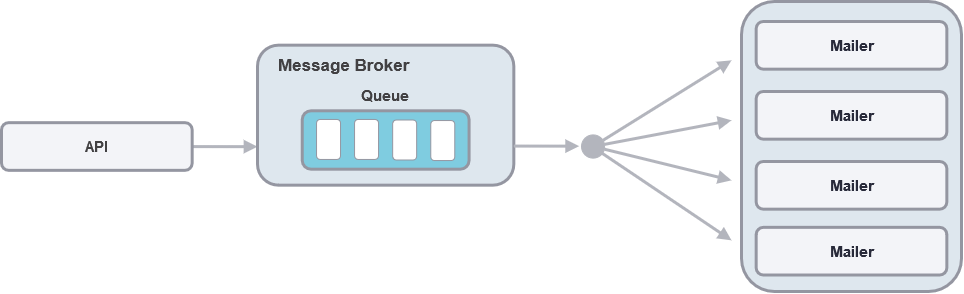
\includegraphics[scale=0.45]{competing-consumer.png}
    \caption{Rappresentazione semplificata del \textit{Competing Consumer pattern}}
    \label{fig:CompetingConsumers}
\end{figure}

Per implementare questo modello si è deciso di utilizzare i seguenti elementi:
\begin{itemize}
    \itemsep0em
    \item \textit{Task Queue}: coda usata per distribuire su più \textit{consumers} varie operazioni che richiedono molto tempo.
    \item Distribuzione \textit{Round Robin}: il broker manderà un messaggio a ogni \textit{consumer} in maniera sequenziale (ogni \textit{consumer} riceverà in media lo stesso numero di messaggi). Questo garantisce che tutti i messaggi verranno recapitati almeno una volta.
    \item \textit{Message acknowledgment} (ACK): vengono utilizzati degli ACK per confermare la corretta elaborazione di un messaggio da parte di un \textit{consumer}. Se l'ACK non viene inviato al broker, il messaggio verrà rimesso in coda.
\end{itemize}
Grazie a questi elementi è stato possibile creare una architettura di messaggistica in grado di scalare orizzontalmente con facilità (aggiungendo dei \textit{consumers}), disaccoppiata, affidabile e resiliente.



